\label{chap:problem_formulation}

This chapter discusses in detail the limitations with current display protocol technology that were alluded to in Chapter~\ref{chap:introduction}. From there, it focuses on how these limitations affect adversely IRLED projector technology. Finally, it provides a problem solution.

\section{Display Protocol Limitations}

    % FIXME: Reference display protocol background section here

    Current display technologies, such as HDMI, assumes a fixed frame rate display which places a hard limit on frame timing and synchronization.

    % Limitations:
    % Synchronization:
    %   -Implementation and integration-costs $
    %   -System-specific solutions $
    %   -Poor upgradeability $
    In detail, the underlying display protocols operate in a best-effort fashion where a buffer swap transmitting a frame of data occurs at static predetermined interval. If a new frame is unavailable to be transmitted at each interval due to any delay, such as processing delay, the previous frame will be retransmitted. This necessarily makes correct synchronization challenging because modern computation systems do not generally provide real-time guarantees for several reasons, such as, variability in work needed for frame generation, CPU scheduling, and I/O delays. Generally, while these challenges can be addressed to some degree, they require custom hardware solutions on top of existing display protocols because end-to-end system synchronization is out of the scope of typical display standards which are designed to push relatively low frame rates over single hardware links. This necessitate designers who need strict control over synchronization to implement custom hardware solutions with high implementation and integration costs. Additionally, because these solutions are custom, they are designed for specific hardware and system configurations resulting in the solution not being universally applicable to other setups as well as lacking an abstraction layer causing poor upgradeability.

    % Limitations:
    % Display Protocols
    %   -Frame rate limits                 -> image size inversely proportional to speed $
    %   -Static Bandwidth Requirements     -> full image transfer $
    %   -Static frame rates                -> 60Hz, 100Hz, etc. $
    %   -Scalability                       -> single scene generator, projector driver $
    %   Diagrams: Bandwidth diagram -- referenced already $
    Additionally, because of the static nature of the transmission interval (e.g. 100Hz), the frame rate cannot be dynamically controlled or changed after initialization. Instead, these protocols have static bandwidth requirements for a given resolution and frame rate of the form found in Table~\ref{tbl:bandwidth}, which shows that image size is inversely proportional to the max speed the display can operate at. Additionally, these protocols only support sending the entire frame at a given interval even if only a small portion of the frame has changed. This is a non-optimal use of bandwidth that does not allow for fine-grained control over the frame rate in cases where a user might wish to dynamically change the frame rate to match the processing rate. In high-speed display scenarios, this inevitably causes frames to be dropped. This issue is further compounded by the fact that traditional display protocols utilize proprietary drivers and hardware such that frame-drops become effectively silent.  Furthermore, because the current protocol scheme is custom tuned for a single hardware setup, this means that generally that the design is not transferable to other setups, such as, ones with a differing number of hardware links; thus, resulting in poor scalability and upgradeability.

    % Analog Chain:
    %   -RT settling time limitations: -- not included right now
    % Existing diagrams:
    %   Diagrams: scene generator -> Non-uniformity Correction -> Projector
    %   Diagrams: Modeline Overhead diagram

    \begin{table}
        \centering
        \large
        %\begin{small}
        %$$bandwidth = resolution \times bits \times fps$$
        %$bandwidth$ : \quad bandwidth requirements in bits per second. \\
        %$resolution$ : \quad number of pixels including porches. \\
        %$bits$ : \quad \quad \quad \ \ \ bits per pixel. \\
        %$fps$ : \quad \quad \quad \ \ \ frames per second.
        \begin{tabular}{| r l |}
            \hline
            $$bandwidth$$ & = resolution $\times$ bits $\times$ fps \\ \hline
            $bandwidth$ & : bandwidth requirements in bits per second. \\
            $resolution$ & : number of pixels including porches. \\
            $bits$ & : bits per pixel. \\
            $fps$ & : frames per second. \\
            \hline
        \end{tabular}
        \caption{Bandwidth requirements of a traditional display protocol}
        \label{tbl:bandwidth}
        %\end{small}
    \end{table}

\section{High-speed IRLED Projector systems}
% How these limitations affect IRSP
% Bottlenecks:
% Hardware limitations:
%   -Physical interconnect bandwidth and latency -> Concurrency/Parallelization $
%   -FPGA/ASIC/IC clock rates                    -> Concurrency/Parallelization $
%   -Analog chain settling times (DAC)           -> Address only the pixels needed $
% Software limitations:
%   -Computational/algorithmic limitations       -> Concurrency/Parallelization $
%   -Poorly optimized software / drivers         -> Don't use $
%   -Fixed frame display                         -> Dynamic frame rate + frame segmentation $
%   -Non-RT scheduling                           -> Realtime schedule / DMA -- not covered below - do i want to cover this?
%   -Lack of control                             -> Use a communication protocol with dynamic control built-in $
%

%FIXME: stick section BLAH in
    In the field, these conventional display protocols, which are designed for driving relatively low speed consumer electronics as indicated in Chapter~\ref{chap:display_protocols}, are often utilized in High-speed IRLED Projector systems. This results in a combination of unnecessary hardware and software limitations being incorporated into systems. This section will discuss these limitations and the general methodology toward alleviating them. Hardware limitations will be discussed followed by software.

    \subsection{Hardware Limitations}
        There are several hardware limitations including physical bandwidth and latency, FPGA, ASIC, IC clock rates, and analog chain settling times. The physical hardware that data is transferred over has inherent characteristics that dictate the maximum bandwidth and latency that cannot be overcome due to the nature of physics. One solution toward, working around this is to introduce more parallel links into a system. A similar issue arises with respect to the clock rates of components within a system, such as, projector driver firmware, and scene generator. Ideally, these components would operate as fast as possible, but reality dictates physical limitations. Similarly introducing more projector drivers, or scene generators could alleviate this issue. The speed of the analog chain in these systems is dictated by the digital to analog converter (DAC) settling times which can in some ways be alleviated by increasing the number of converters utilized within a system. This allows each DAC to drive a smaller portion of an array.

    \subsection{Software Limitations}
        In terms of software, computational and algorithm limitations exist in the generation of scenery for display, and in correcting for pixel and array imperfections as well as in putting data in the correct format to be understood by a projector's driving firmware. Rendering of individual frames of a scene can be particularly computationally expensive. This can be further complicated by poorly optimized software drivers or algorithms. Additionally, in these systems, tight control over timing is important because frame drops are not tolerable. Meaning that fixed rate display technology is a hinderance in terms of user level control. One solution toward that is to utilize technology that allows dynamic frame rates and frame segmentation, which, requires protocols with dynamic control built in.


\section{Problem Statement}
    IRSP systems need to be capable of operating at high speeds with large resolutions. Typically, this can be on the order of 2048 by 2048 and up to 1KHz frame rates end-to-end with low subframe latency. Necessarily, these goals represent a challenging problem to overcome when utilizing typical display technology which is furthered due to the limitations discussed above. Given these goals, what are appropriate solutions for addressing the issues with current display technology? The central question we could ask ourselves is, how to architect a dynamic scalable IRLED projection end-to-end system capable of High-performance operation, sub-frame latency, dynamic frame rates, intelligent Bandwidth utilization, intelligent DAC utilization as well as upgradeability and generalizability?

\section{Problem Solution}
    Within the current display protocol technology, any effort to address the aforementioned issues requires system developers to have complete control over an entire end-to-end system for the solution to operate correctly. This means that in practice customized hardware and software that deviates from the standard display protocols behavior is required. Any solution, that lacks these requirements would fail to completely address the issue.

    In short, to truly address issues within the traditional display protocol would require creating a new system specific protocol tied to specific custom hardware. Additionally, with this type of solution, it is still not possible to achieve true sub-frame latencies due to the nature of display protocols transmitting requiring transmission of entire frames of data at a given interval or frame rate.

    I believe that any effort to address the aforementioned issues and answer our problem statement requires developing an alternative display protocol designed specifically for high-speed low latency frame transmission as well as is hardware agnostic in nature, and utilizable within different types of hardware setups. This would allow for the protocol be retrofitted within existing systems as well as allow for upgradeability, and support for future hardware. In order, to achieve sub-frame latencies, this protocol would need to support transmission of sub-frames of data, i.e. transmission of partial frames. Allowing for partial frame transmission enables a host of other desirable features, such as, the ability to control bandwidth utilization and the ability to incorporate dynamic frame rates. A good method of supporting partial frame transfer is to utilize headered packets of data to provide a context for what the data represents and where to draw said data on a display. This novel method of transferring display data is called a packetized display protocol (PDP).

    As discussed briefly in the Chapter~\ref{chap:introduction}, my PDP architecture eschews with assumptions found in traditional display technologies to provide a robust feature-set. This section discusses many of the assumptions of traditional display technologies and how the PDP architecture differs, in order to provide the reader with an understanding of the benefits to proposed alternative technology.

    In contrast to a normal display protocols, the proposed architecture, is designed to utilize a dynamic source driven refresh rate through the coordination of both source (scene generator) and sink (display). In this architecture, frames are segmented into pieces or sub-frames and sent to the display based upon how often these segments need to update. An example of this is shown in Figure~\ref{fig:variable_display} where different regions of the display operate at different frame rates. By utilizing dynamic frame rate control at sub-frame resolutions, substantial bandwidth reductions can occur. This will be discussed in further detail in subsequent chapters.

    \begin{figure}
        \centering
        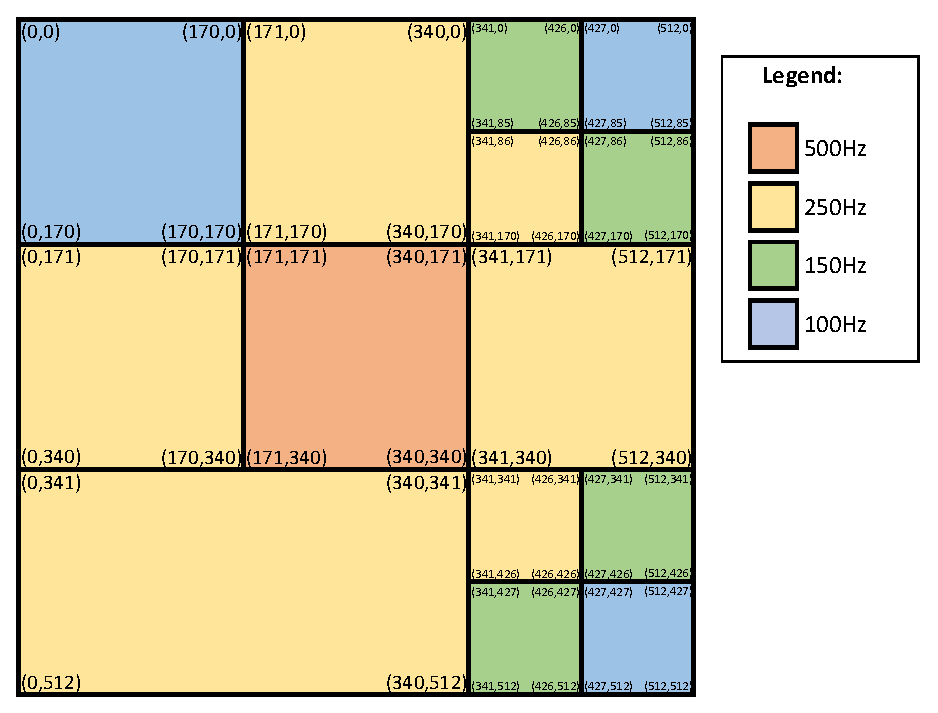
\includegraphics[width=1.0\textwidth]{fig/variable_display.pdf}
        \caption{Dynamic frame rate display with multiple regions updating at different frame rates}
        \label{fig:variable_display}
    \end{figure}

    %FIXME: what mechanisms to synchronize displays?
    As will be discussed in Chapter~\ref{chap:pdp_protocol}, the underlying PDP protocol itself is designed to allow for fine-grained control over when and what data is transmitted as well as incorporate mechanisms to synchronize displays. Furthermore, the protocol architecture is abstracted in such a way that the physical interconnect layers are transparent in order to enable it to be capable of operating over a wide-spectrum of hardware as well as to allow the protocol to be extended and used within future hardware. This allows for risk reduction because it allows simpler migration to new platforms as new hardware becomes available. For example, a hardware system implementing this protocol could switch or upgrade physical components and still utilize the same protocol within the software stack given an appropriately compatible physical layer. To further facilitate this, a packetized protocol structure capable of transmitting pixel data in a generalized way has been chosen. will discuss the architecture of the protocol.
